\chapter{Iteration Plan 2 (FYP 1 Final)}
\label{ch:iter2}

The second iteration plan for our project is explained in this chapter. This chapter will provide guidance on the project’s modules and their development. Students are expected to talk about the project’s second stage of method of implementation in this chapter:

\section{FYP 1 Final:}
\begin{itemize}
    \item FYP 1 Final Presentation: \begin{itemize}
    \item Environment setup in Unity3D and Blender 
    \item Designed basic environment of Hospital
    \end{itemize}
\end{itemize}

\section{Designed basic environment of Hospital:}
	\begin{itemize}
	\item Reception Area
	\item Waiting Rooms
	\item Patient Rooms
	\item Training Facilities
\end{itemize}	
	
\subsection{Hospital Entrance:}
The hospital entrance serves as the main entry point to the virtual hospital
	\begin{figure}[h]
		\centering
		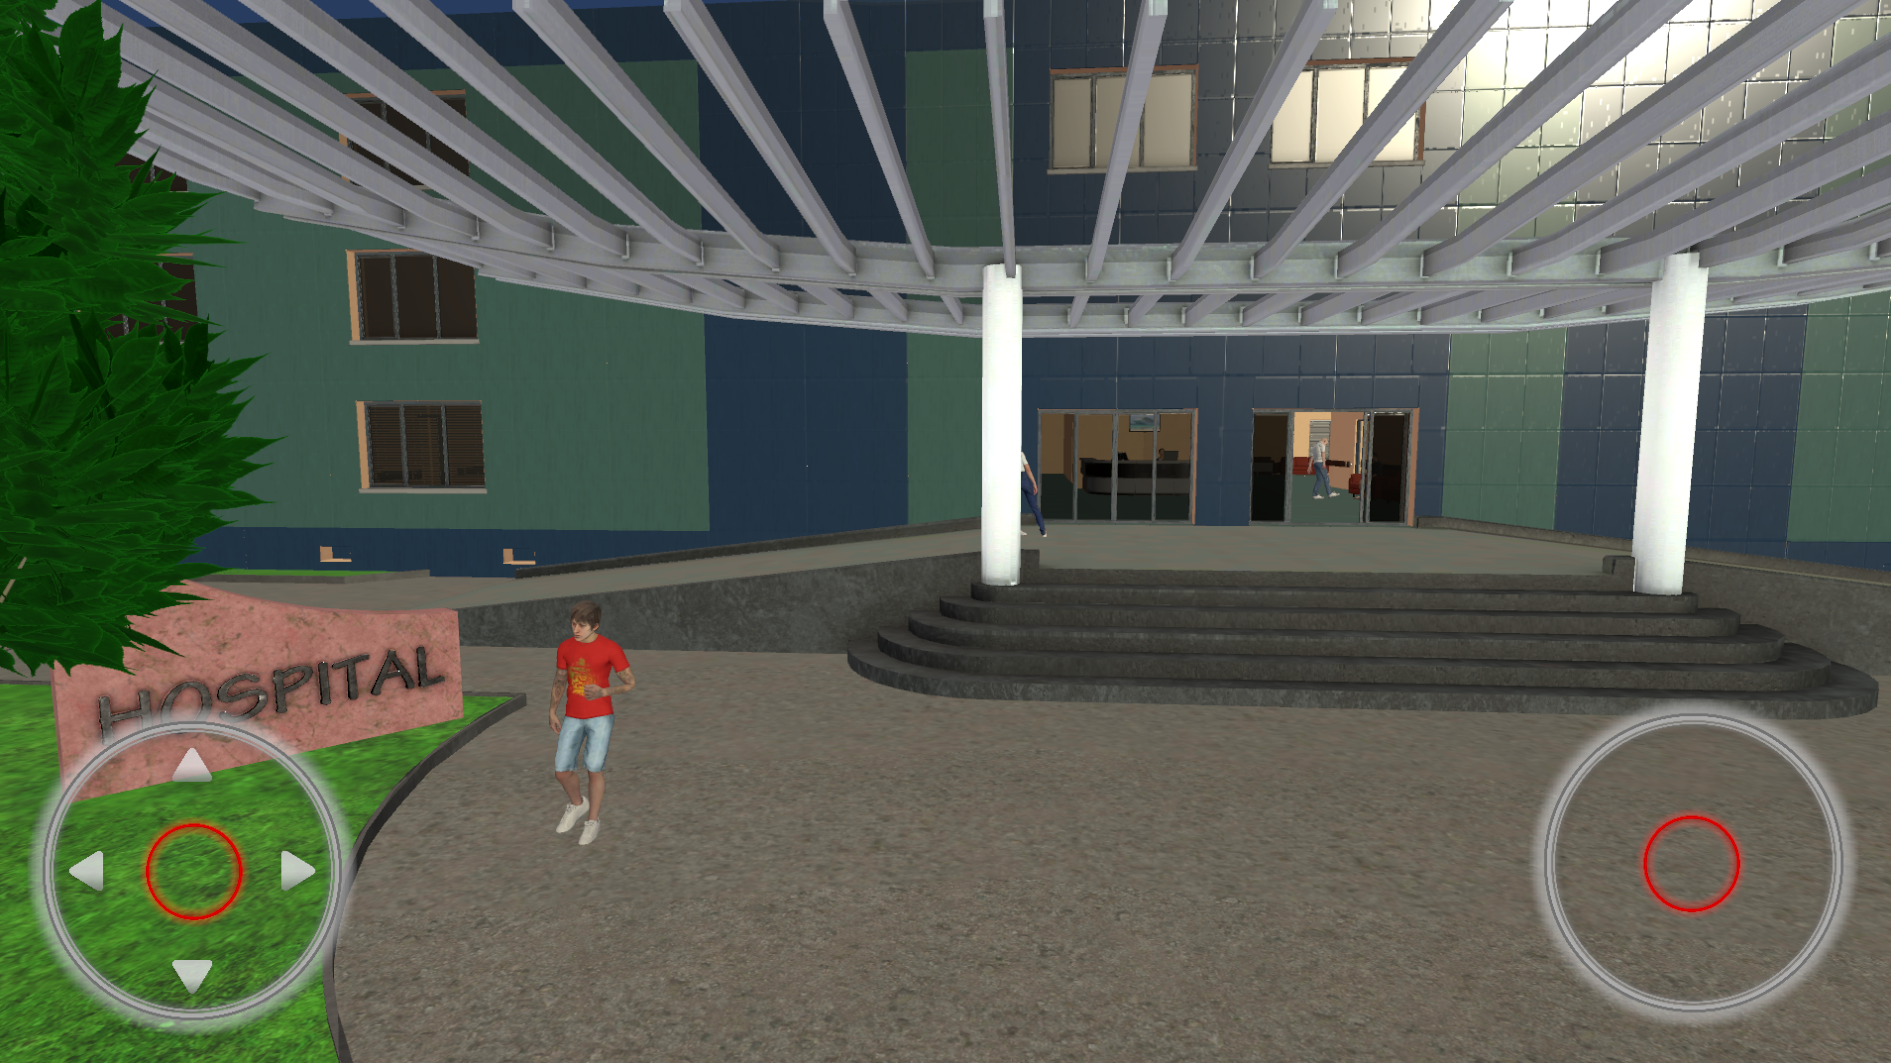
\includegraphics[width=0.5\textwidth, height=0.3\textheight]{Images/Hospital Enterance.png}
		\caption{Hospital Enterance}
		\label{fig:system-diagram}
	\end{figure}
\newline

\subsection{Reception Area:}
The reception area serves as the main entrance point to the virtual hospital. Where virtual receptionists greet patients and visitors. Patients can check-in here, provide necessary information.
\begin{figure}[h]
	\centering
	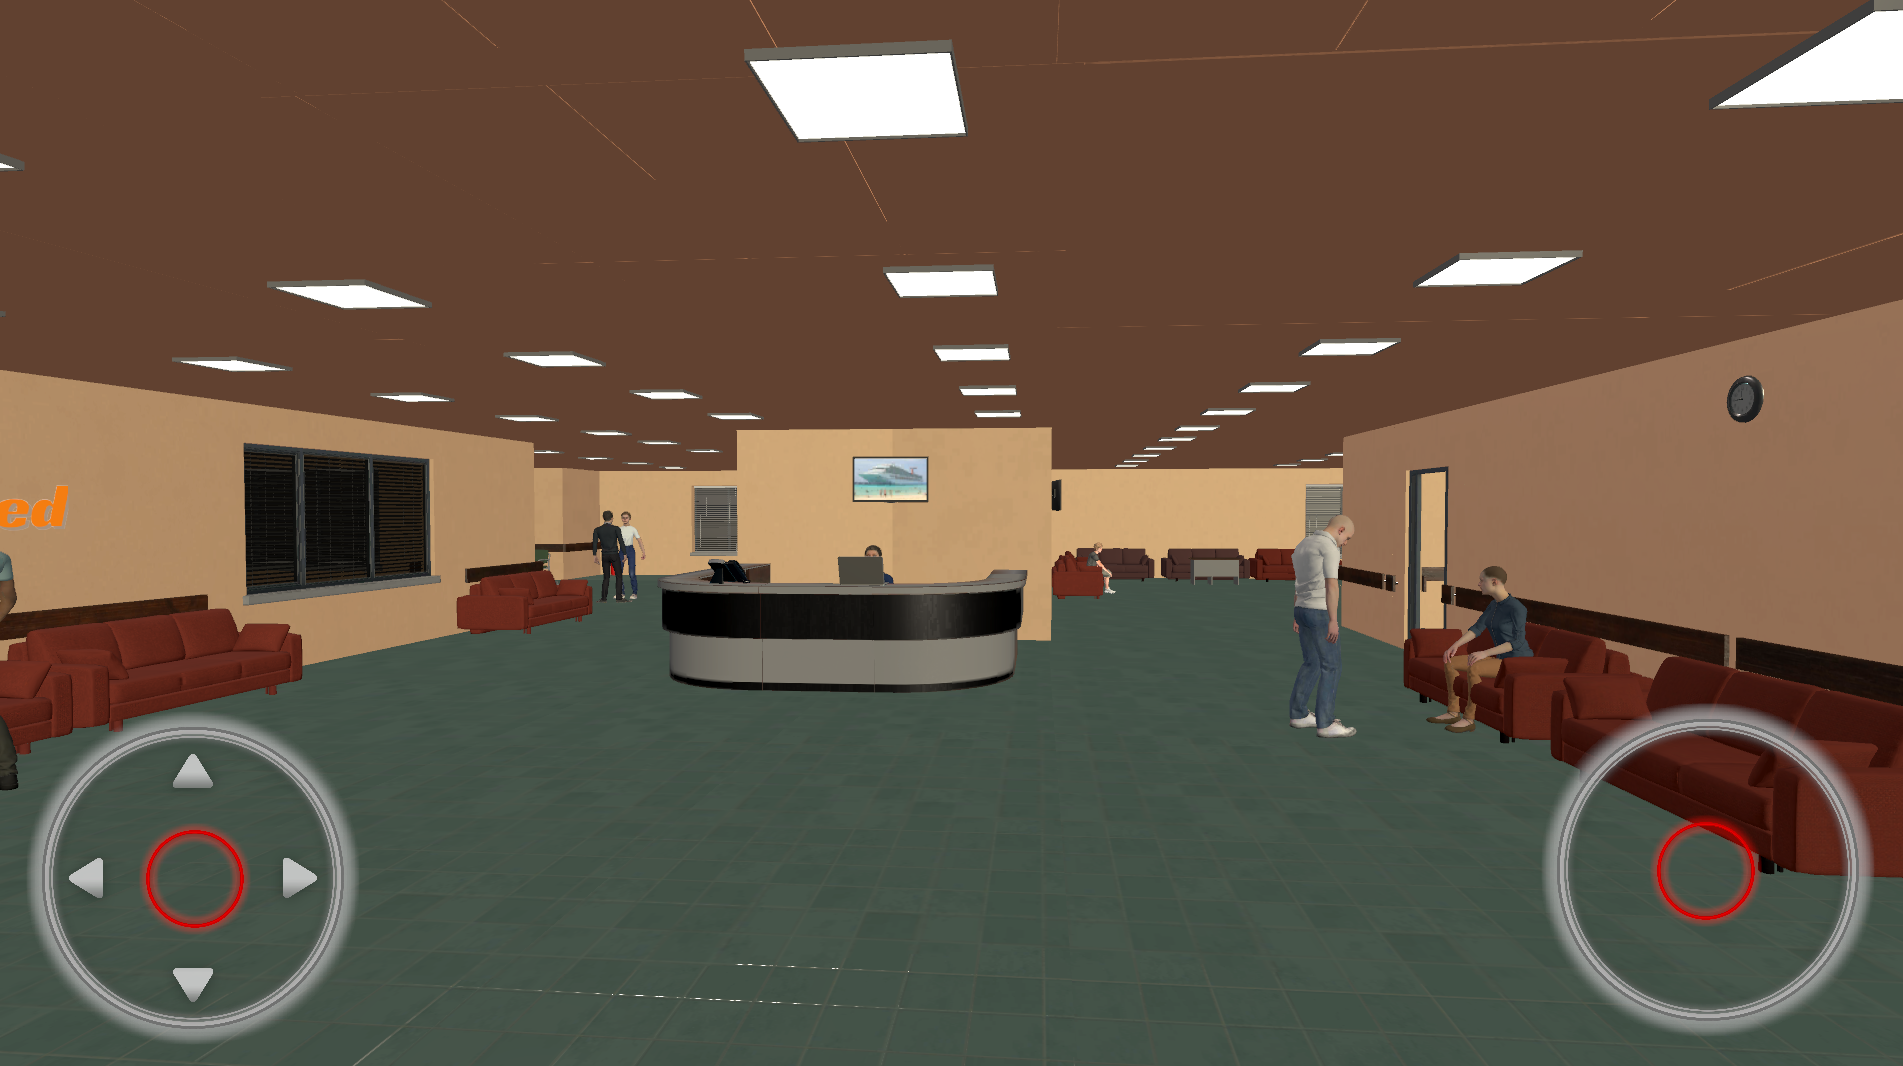
\includegraphics[width=0.5\textwidth, height=0.3\textheight]{Images/Reception Area.png}
	\caption{Reception Area}
	\label{fig:system-diagram}
\end{figure}
\newline

\subsection{Waiting Area:}	
Waiting area is designed to provide comfortable seating arrangements for patients and their companions while they wait for appointments or procedures.
\begin{figure}[h]
		\centering
		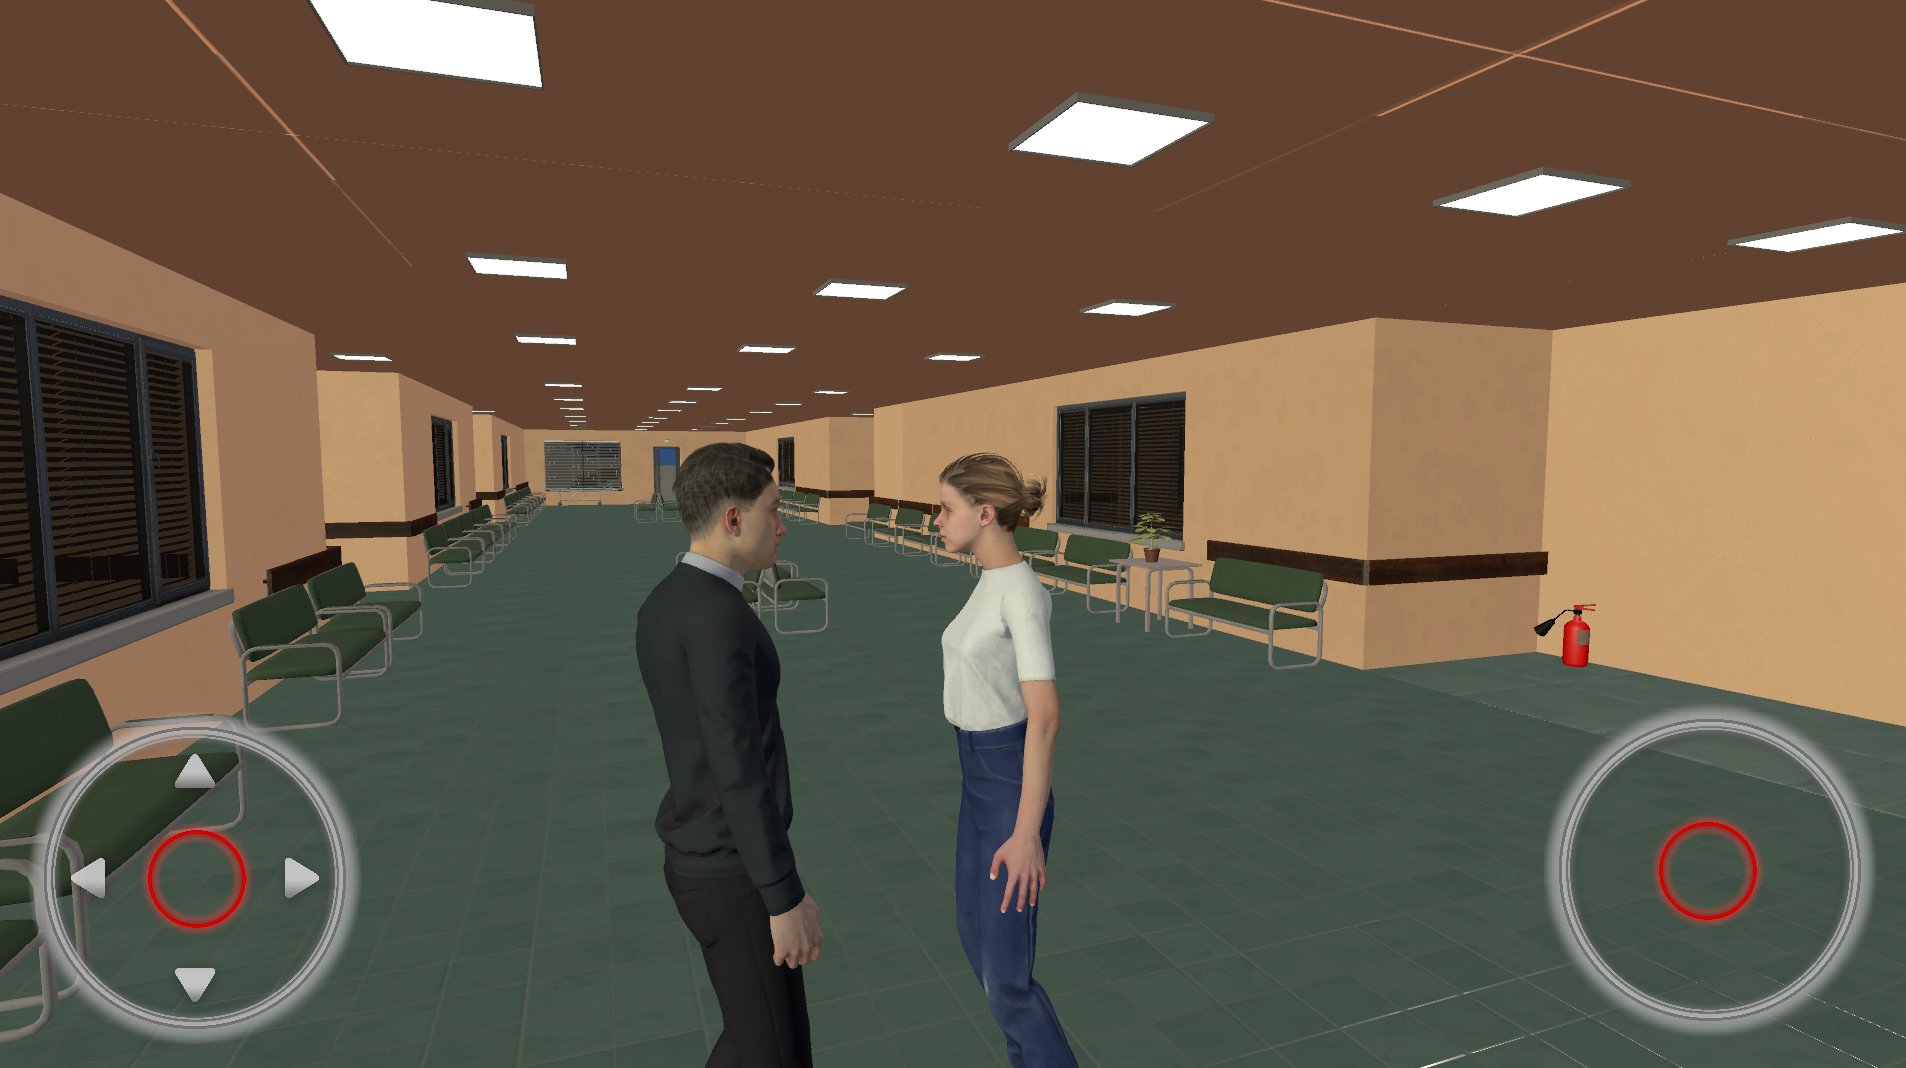
\includegraphics[width=0.5\textwidth, height=0.3\textheight]{Images/Waiting Area.png}
		\caption{Waiting Area}
\end{figure}
\\
\subsection{Patient Rooms:}	
Patient rooms are designed to provide a comfortable and healing environment for patients during their hospital stay.
	\begin{figure}[h]
		\centering
		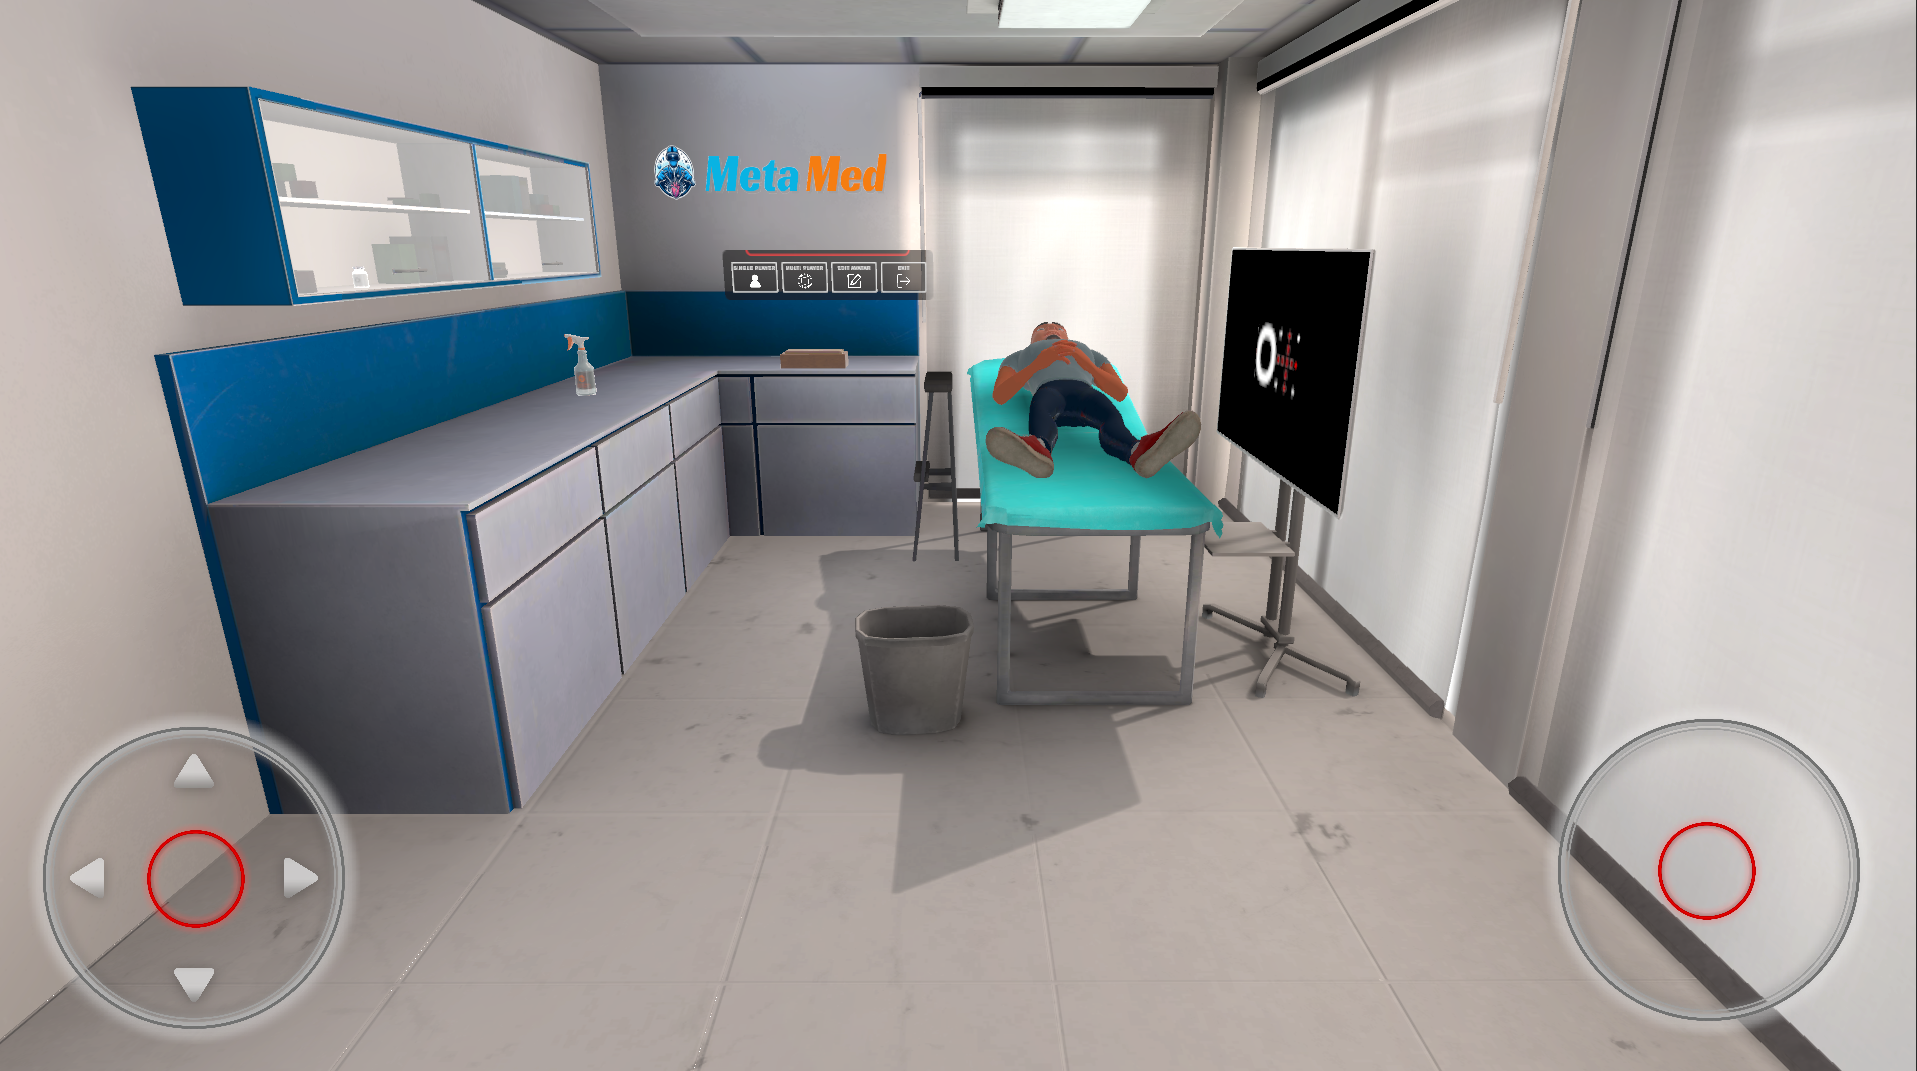
\includegraphics[width=0.5\textwidth, height=0.3\textheight]{Images/Patient Room.png}
		\caption{Patient Room}
		\label{fig:Patient-Room}
	\end{figure}	

\subsection{Patient Body:}	
We created Patient Body in Metaverse Hospital to simulate patient interactions, provide realistic medical scenarios for training, and enhance learning experiences for healthcare professionals in a virtual environment.
\begin{figure}[h]
	\centering
	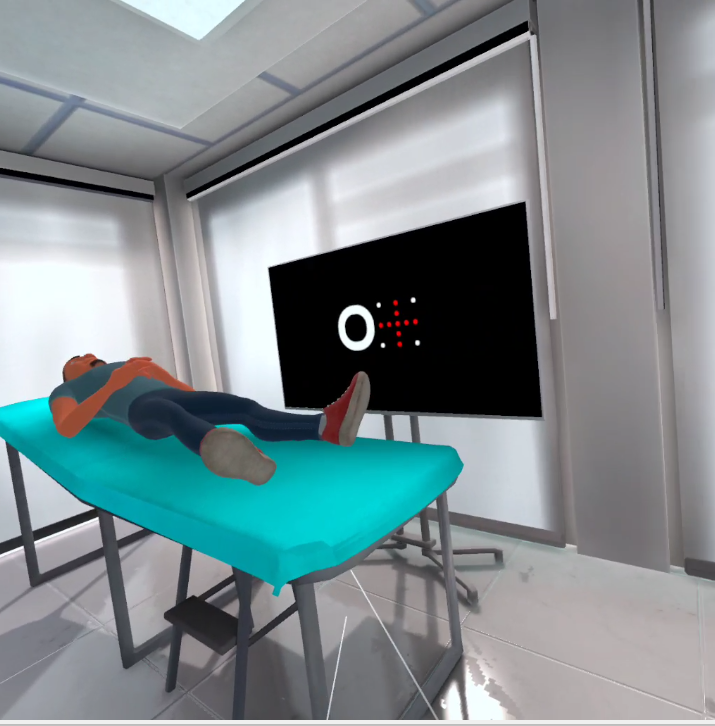
\includegraphics[width=0.5\textwidth, height=0.3\textheight]{Images/Patient Body.png}
	\caption{Patient Room}
	\label{fig:system-diagram}
\end{figure}	

	